\subsection{Reconocimiento de rostros}

Un aplicación fue el uso de los servicios de detección de rostros y reconocimiento de sujetos de la API de Kairos en una aplicación móvil. Ésta permite que los usuarios
ejecuten un potente recurso en la nube para reconocimiento
de caras enviando sólo una imagen capturada por el robot.

\subsubsection{Objetivos}

\begin{itemize}
    \item Integrar un servicio en la nube con una aplicación
    en la robótica móvil.
    \item Crear una interfaz simple y amigable para que cualquier usuario acceda a la funcionalidad del reconocimiento de rostros.
    \item Utilizar una alternativa a la API de \texttt{ALFaceDetection}.
\end{itemize}

\subsubsection{Problema}

El robot Fibonacho, a través de la API de NAOqi \texttt{ALFaceDetection},
cuenta con métodos que permiten la detección de rostros
y el reconocimiento de caras previamente almacenadas.
La detección de rostros se ejecuta lo suficientemente rápido como
para poner en funcionamiento un rastreador o seguidor
de rostros. El reconocimiento de personas lleva casi el 
mismo tiempo de procesamiento y funciona a pesar de algunas
variaciones en las caras, por ejemplo, si el sujeto lleva 
una gorra o lentes.

Aunque la API de NAOqi funciona muy bien, tiene
algunas desventajas como: guardar en el disco del robot la foto de un 
rostro para su futuro reconocimiento, el proceso de aprendizaje 
de nuevas personas no es simple para usuarios inexpertos
y no aprovecha más información ofrecida en la imagen.

\subsubsection{Solución}

Hay varias plataformas para detección de rostros, pero 
se eligió Kairos por todas las características que ofrece
gratis a los desarrolladores.
A través de la API de Kairos tenemos acceso
a funcionalidades que son parte de la solución 
a los problemas que no abarca \texttt{ALFaceDection}.
Se guardan en la nube las imágenes de nuevos sujetos
detectados y añadir una nueva cara se hace
con una simple petición al recurso \texttt{enroll}.
Kairos también permite analizar la imagen para detectar el género, 
edad o raza de las personas.

En la API REST se utilizan los servicios de detección de rostros y reconocimiento
de sujetos de la API de Kairos.
Dentro de la aplicación móvil, la API REST es el intermediario
que se comunica con la API de Kairos, esto es por facilidad y por no
tener que manejar muchas API y SDK por cada servicio que se desee usar.
% A pesar de que en el sistema sólo se utiliza el servicio
% dentro de la aplicación móvil, es posible ejecutar directamente la clase
% \texttt{Kairos} del módulo \texttt{app.tpa\_client\_libraries.kairos\_client}
% en el robot (esta clase es parte del la API REST de CloudNAO), para enviar la petición y procesar la respuesta desde éste.
% Por ahora sólo se muestra el uso de este servicio en la aplicación móvil.

\begin{figure}[htbp]
    \centering
    \subfloat{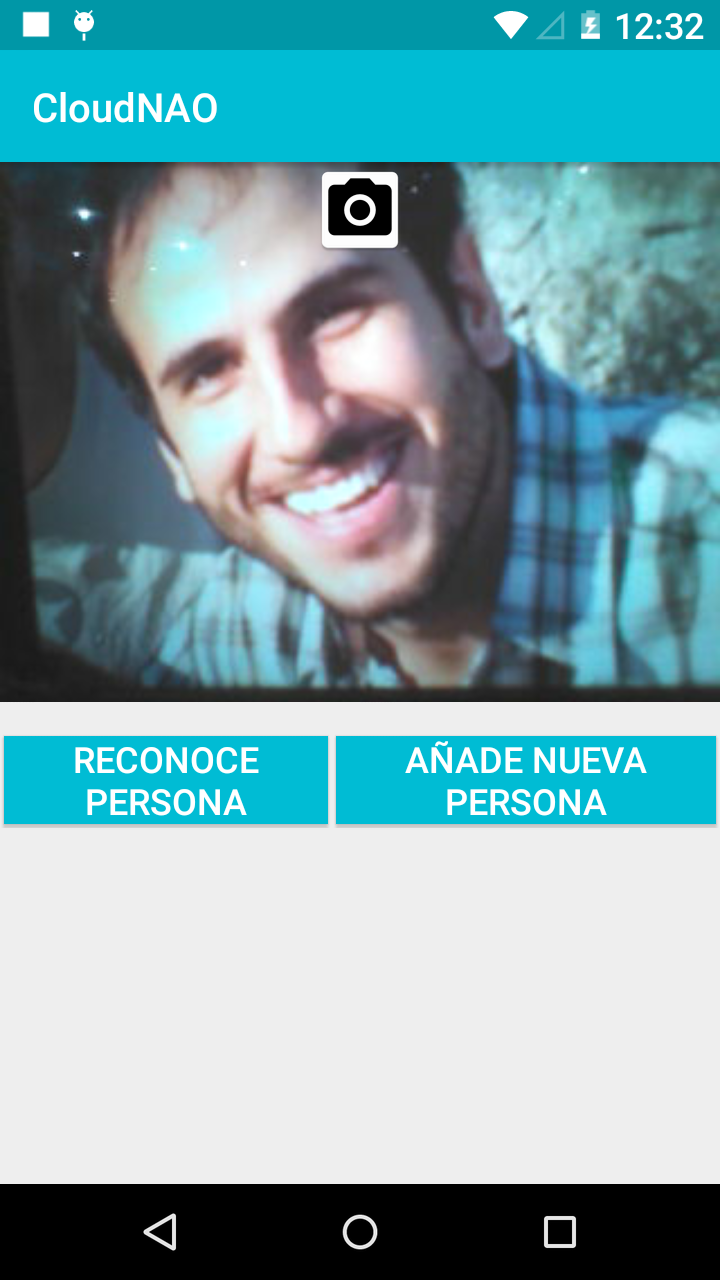
\includegraphics[scale=.1]{face_study_case1}}%
    \qquad
    \subfloat{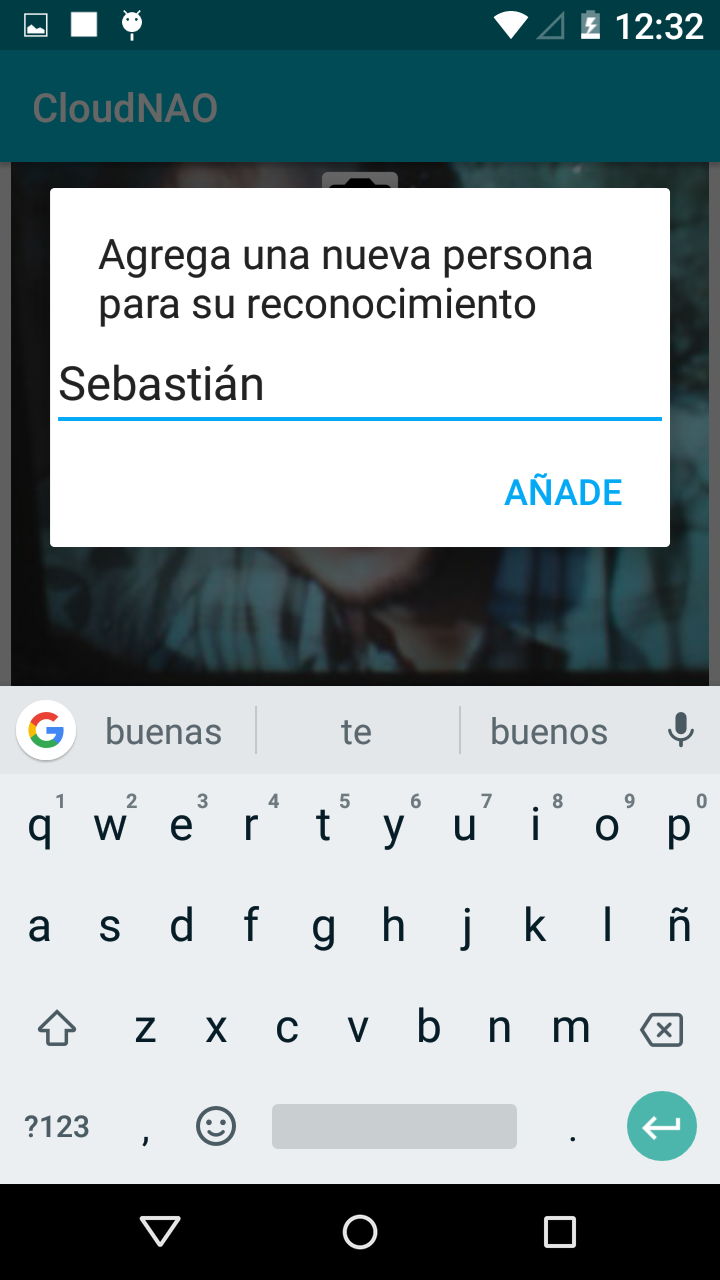
\includegraphics[scale=.1]{face_study_case2}}%
    \qquad
    \subfloat{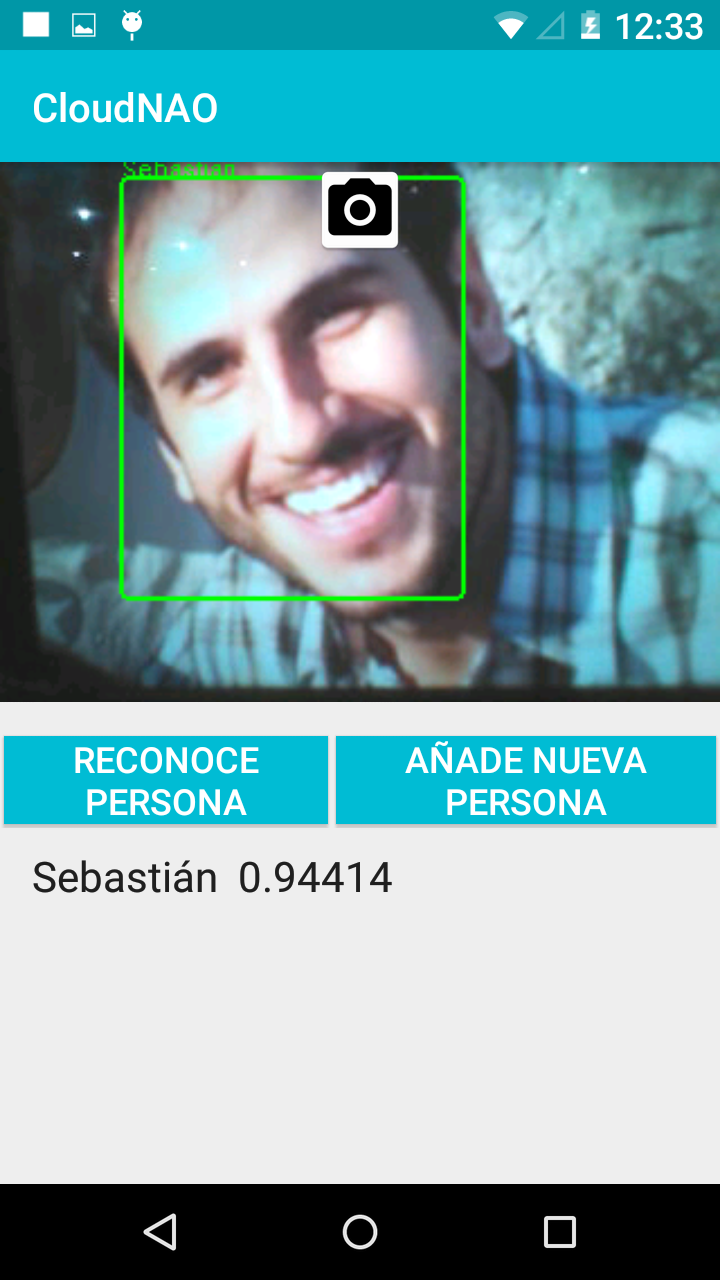
\includegraphics[scale=.1]{face_study_case3}}%
    \caption{Ejemplo de cómo se registrar un nuevo sujeto para su posterior reconocimiento.}
\end{figure}
Cuando el usuario selecciona en el menú de navegación de la aplicación
la tarea de \textbf{Reconocimiento de personas} se muestra una pantalla 
con tres botones, uno para obtener una fotografía del robot, otro para
detectar rostros de nuevas personas, y el tercero para reconocer sujetos
ya almacenados. Si el usuario desea añadir a una nueva persona, se abre un
formulario emergente con un campo para agregar el nombre de la persona y
si no hay errores y la detección se realizó correctamente,
la cara de la persona queda almacenada y se pueden realizar futuros reconocimientos.
Si se desea realizar el reconocimiento de personas cuyo rostro
fue previamente guardado, se presiona el botón con la etiqueta
\textit{Reconoce personas} y si todo sale bien,
se muestra una lista de las personas en la fotografía.
Al dar clic sobre el nombre de la persona en la lista, el robot ejecuta
un movimiento de saludo diciendo una frase simple con el nombre de la persona.



\subsubsection{Resultados}

La velocidad de la ejecución de la tarea
depende mucho de la conexión a internet.
El ejemplo en el que se ocupa el reconocimiento
de rostros es bastante sencillo, el robot
sólo hace un gesto de saludo. No obstante 
podemos añadir más funcionalidades donde
aprovechemos el análisis completo que ofrece
Kairos, la detección del género, la edad y la raza.



\begin{figure}[htbp]
\centering
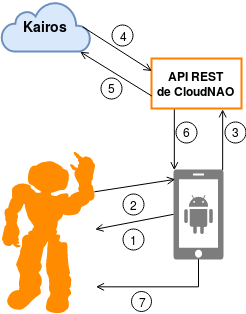
\includegraphics[scale=0.6]{study_case_kairos}
\caption{El flujo de el reconocimiento de personas. 1) El usuario presiona el botón para capturar una imagen desde el robot. 2) El robot envía la imagen a la 
aplicación. 3) El usuario presiona el botón Reconoce personas y envía la imagen a la API REST. 4) La API solicita el recurso \texttt{recognize} de Kairos. 5) Kairos envía un JSON como respuesta. 6) La API 
envía un JSON a la aplicación móvil. 7) La aplicación ejecuta remotamente el módulo de NAOqi para realizar el discurso animado.}
\end{figure}



\subsection{Reconocimiento óptico de caracteres y traducción de texto}

Una aplicación interesante es la
detección de texto en una imagen y su
traducción.
En la API REST se combinan dos servicios
para añadir al robot Fibonacho la funcionalidad de extracción y traducción de texto en imágenes. 


\subsubsection{Objetivos}

\begin{itemize}
    \item Implementar el reconocimiento óptico
    de caracteres sobre el robot Fibonacho.
    \item Utilizar servicios en la nube para traducción
    automática neuronal y reconocimiento óptico de caracteres.
    \item Permitir que el robot asista a los usuarios
    en la traducción de texto encontrado en una imagen.
\end{itemize}

\subsubsection{Problema}

El reconocimiento óptico de caracteres (OCR por sus siglas en inglés) permite detectar y extraer texto de imágenes para luego
almacenarlo en un formato que una máquina pueda entender.

A diferencia del caso de estudio anterior, el robot Fibonacho
no cuenta con una API para detección de
texto en imágenes, ni con una herramienta
para traducir sentencias. Por las características
del robot, la interacción con humanos es 
amigable, por lo que una funcionalidad como la de asistir
a los usuarios en la traducción de texto a través
de imágenes tiene una amplia aplicación.

\subsubsection{Solución}


La API de Vision de Google Cloud ofrece el servicio de OCR
que además incluye la detección del idioma en que se encuentra escrito el texto encontrado.
Google Cloud cuenta también con una API para traducción de 
texto.
En la API REST se combinan estos dos servicios
para añadir al robot Fibonacho la funcionalidad de extracción y traducción de texto en imágenes. 

El usuario simplemente adquiere una fotografía
capturada por la cámara del robot y se hace la petición
a la API REST que utiliza los servicios
de Google Cloud Vision y Translation para obtener el texto
y hacer la traducción, respectivamente.
Si existe texto en la imagen y fue correctamente procesado por
la API de Vision, éste se traduce, el resultado se muestra
en la aplicación y el robot repite oralmente
el texto traducido.

\subsubsection{Resultados}

Gracias a los servicios utilizados, la traducción 
del texto en una imagen se resuelve fácilmente.
La aplicación ofrece una interfaz fácil para cualquier
usuario. El tiempo de ejecución de la tarea
es de unos cuantos segundos (entre 5 aproximadamente), aunque es
una variable dependiente de la velocidad de la conexión 
a internet.


\begin{figure}[htbp]
    \centering
    \subfloat{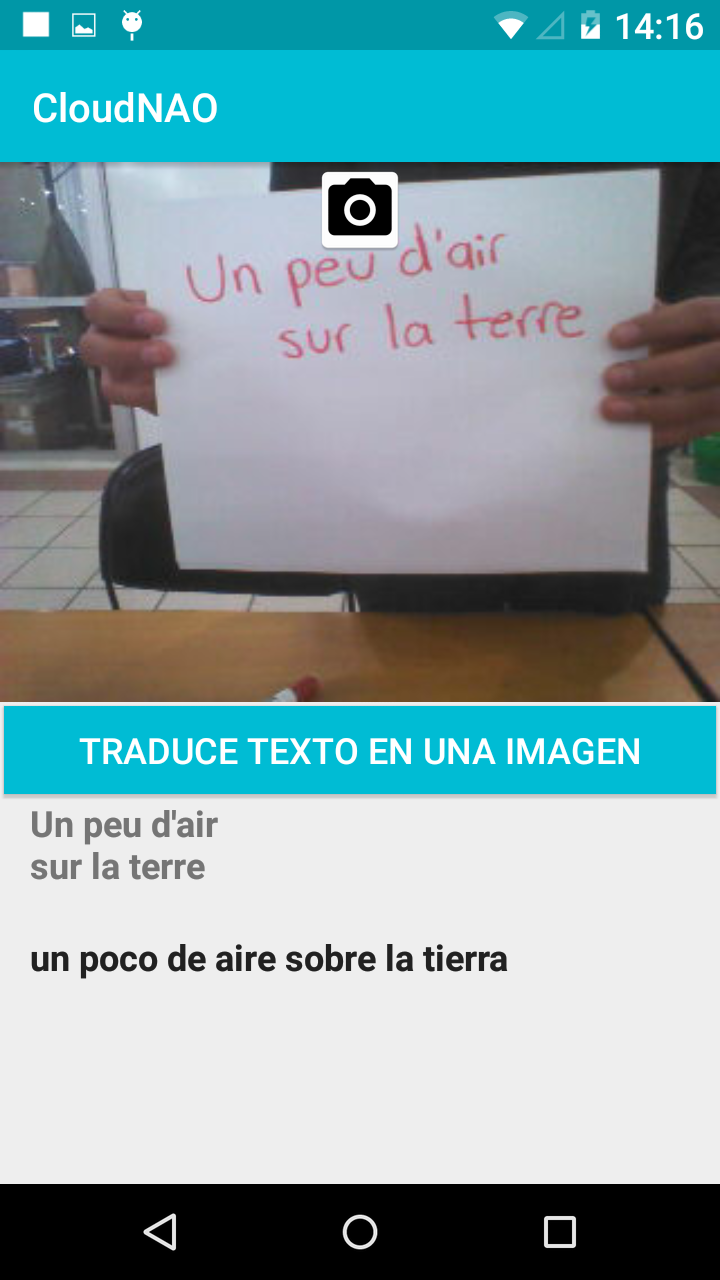
\includegraphics[scale=.1]{ocr_study_case1}}%
    \qquad
    \subfloat{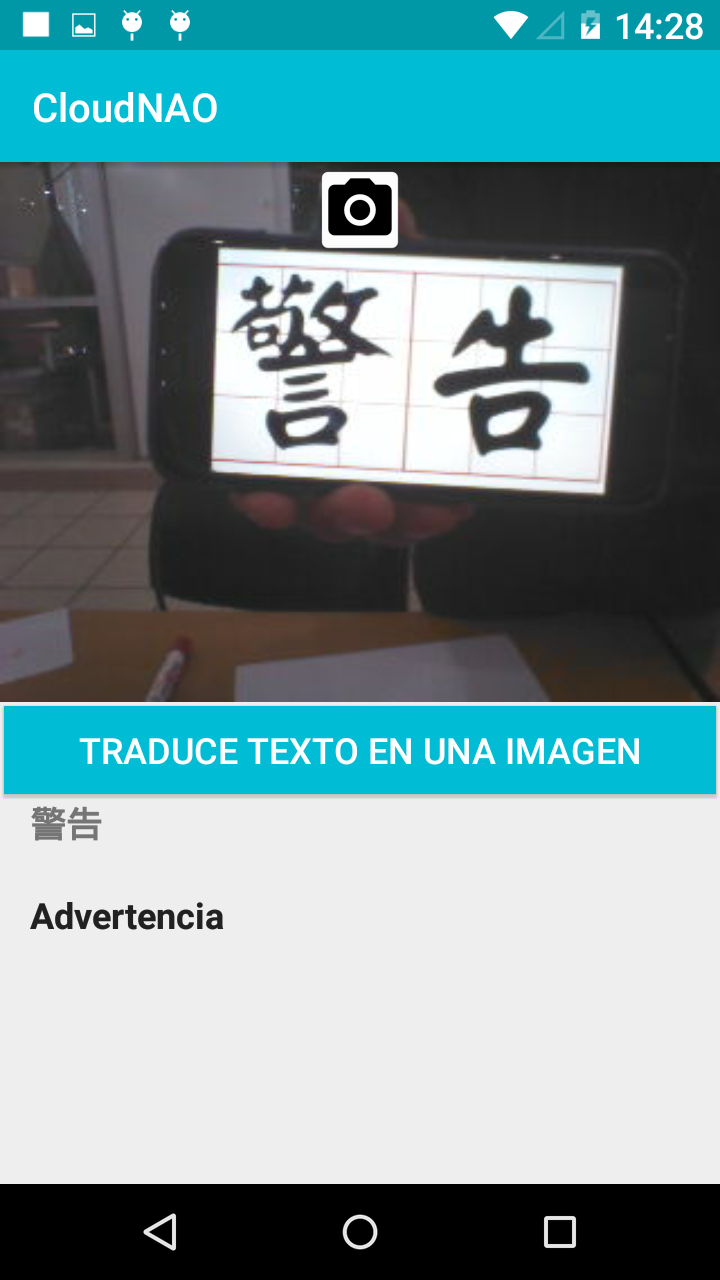
\includegraphics[scale=.1]{ocr_study_case2}}
    \caption{Ejemplo de la traducción
    de dos sentencias, la primera en francés y la segunda
    en chino.}
\end{figure}

\subsection{Reconocimiento de voz}

Este caso de estudio se aplica
directamente sobre el robot Fibonacho, conectándolo
a la API de Wit.ai para procesamiento de
un discurso oral y poder interactuar con él a través de comandos de voz.


\subsubsection{Objetivos}

\begin{itemize}

    \item Utilizar un servicio de procesamiento
    de lenguaje natural en la nube.
    \item Desarrollar un asistente sencillo con una interacción por voz sobre el robot Fibonacho.
    \item Implementar en el robot, un programa local
    que se conecte con servicios en la nube.
    
\end{itemize}

\subsubsection{Problema}


Una aplicación interesante de tecnologías que realizan el
procesamiento de lenguaje natural es la creación de bots conversacionales
o asistentes por voz.
El robot Fibonacho es una plataforma con las características
para servir como asistente por voz, que a pesar de contar con un
módulo de reconocimiento de voz (\texttt{ALSpeechRecognition}), éste es muy 
básico y limitado.

Una aplicación de reconocimiento de voz
utilizando únicamente la API de NAOqi es estática.
El módulo \texttt{ALSpeechRecognition} sólo reconoce
palabras predefinidas no la intención
del discurso del usuario.
Por ejemplo, si deseamos que el robot salude
cuando un usuario lo hace, se deben 
definir todas las formas posibles en las que
la persona puede decir ``Hola''.

\subsubsection{Solución}

Wit.ai provee una API para construir aplicaciones
con las que los usuarios se puedan comunicar a través de voz o texto.
Las aplicaciones desarrollados con Wit.ai aprenden conforme reciban más 
información, se vuelven más inteligentes con cada interacción de los usuarios.

Se creó una aplicación sencilla
para interactuar con el robot usando el servicio \texttt{speech} de
Wit.ai.
Dentro de la API REST existe un módulo para hacer las peticiones
a la API de Wit.ai. Éste también puede usarse directamente sobre
el robot, evitando un intermediario.
Se solicita el recurso \texttt{speech} de la API de Wit.ai 
enviando
un archivo de audio generado por el robot. La API
envía como respuesta un JSON con la transcripción del audio 
en texto, las entidades e intenciones encontradas.
El robot es quien se encarga de manejar el flujo de
acciones dependiendo de las intenciones.

Las intenciones y entidades de una aplicación se definen en la plataforma
web de Wit.ai. Ésta cuenta con una herramienta para
crear estos dos elementos a partir de oraciones que el usuario
posiblemente enviará en un mensaje. Por ejemplo,
cuando el usuario inicie una conversación posiblemente
sea con un ``Hola robot'', por lo que podemos definir una
intención con valor \texttt{saludo}.
Se pueden añadir más sentencias
que correspondan a la intención \texttt{saludo}
como ``Buenas tardes'' o
``Buena día Fibonacho''.
La entidades permite realizar específicamente cierta acción.
Por ejemplo, si le decimos: ``Cambia a la posición de descanso'', la intención es \texttt{cambiar posición} y la
entidad es a qué posición debe cambiar, a la de descanso
en nuestro ejemplo.
A partir de esto podemos definir acciones muy simples
para el robot guiadas por las intenciones y entidades. En la tabla \ref{table:intents-study-case} se describen las intenciones y entidades que se
definieron para esta aplicación
y un ejemplo de lo que puede decir el usuario para ejecutar la acción asociada con la intención.

\begin{table}[ht]
\centering
\caption{El valor de la entidad en la sentencia
del usuario se encuentra subrayado.
\label{table:intents-study-case}}
\begin{tabular}{|l|l|l|}
\hline
Intención                                                           & Entidades                                                        & \begin{tabular}[c]{@{}l@{}}El usuario\\ puede decir ...\end{tabular}    \\ \hline
\begin{tabular}[c]{@{}l@{}}CAMBIAR\\ POSTURA\end{tabular}           & postura                                                          & \begin{tabular}[c]{@{}l@{}}Ve a la posición\\ de \underline{descanso}\end{tabular} \\ \hline
CAMINAR                                                             & dirección                                                        & \begin{tabular}[c]{@{}l@{}}Camina hacia\\ la \underline{derecha}\end{tabular}      \\ \hline
INICIO                                                              & nombre del usuario                                               & \begin{tabular}[c]{@{}l@{}}Hola NAO, me llamo\\ \underline{Ivan}\end{tabular}      \\ \hline
FIN                                                                 &                                                                  & Adiós robot                                                            \\ \hline
\begin{tabular}[c]{@{}l@{}}PROCESAMIENTO\\ DE IMÁGENES\end{tabular} & \begin{tabular}[c]{@{}l@{}}tipo de \\ procesamiento\end{tabular} & Lee el \underline{texto}                                                           \\ \hline
\begin{tabular}[c]{@{}l@{}}GUARDA\\ IMÁGENES\end{tabular}           & \begin{tabular}[c]{@{}l@{}}número de\\ fotografías\end{tabular}  & Toma \underline{diez} fotos                                                        \\ \hline
\end{tabular}
\end{table}



% \begin{itemize}
% \item  \texttt{walk}: El robot camina una pequeña distancia. ``Vamos, camina.''
% \item \texttt{restPosition}: El robot cambia a una posición de descanso (crouch). "Descansa robot".
% \item \texttt{greeting}: El robot realiza un gesto y saluda al usuario."Hola robot".
% \item \texttt{photography}: El robot toma una fotografía y la almacena en su disco. "Toma una foto de lo que ves".
% \item \texttt{stop}: El robot se despide del usuario va a una posición de
% descanso y termina la aplicación. "Adiós robot".
% \item \texttt{animation}: El robot ejecuta una animación aleatoria.
% "Robot, dame un movimiento sorpresa".
% \item \texttt{textDetection}: Utilizando la API de Vision de Google Cloud
% el robot extrae texto de una imagen y lo expresa oralmente. "Lee que dice
% aquí".
% \end{itemize}

\subsubsection{Resultados}

Pese a ser una aplicación muy simple
se puede volver tan compleja como se desee,
el añadir más entidades hace más interesante interactuar con el
robot. Podemos agregar otros servicios para
que cada vez se parezca más a un asistente por voz,
como los calendarios y contactos de Google, la búsqueda de lugares y
zonas de interés con servicios como Foursquare o los Mapas de Google,
uso de la la gráfica de conocimiento de Google o de Wolfram Alpha, 
servicios de noticias, etc. El robot no pone las limitaciones 
de la aplicación, ya que éste solamente es una interfaz
entre los servicios en la nube y los usuarios.

\begin{figure}[htbp]
\centering
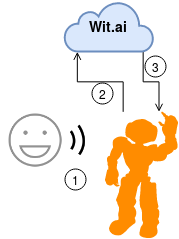
\includegraphics{study_case_wit}
\caption{El funcionamiento de la interacción con el robot a través de un discurso
oral. 1) El usuario envía un mensaje que el robot graba en un archivo de audio de 3 segundos de duración. 2) El robot envía el archivo binario de audio
a la API de Wit.ai. 3) Wit.ai envía un JSON con las entidades encontradas. El robot realiza una acción dependiendo de las entidades.}
\end{figure}

% \subsubsection{Clasificación de imágenes en escenarios}


% Para completar la arquitectura CloudNAO falta implementar un modelo de aprendizaje 
% profundo que se brinde como un servicio web para ser consumido por robots NAO.
% A pesar de que el servicio de detección de objetos es mantenido por el LAR, y 
% se adaptó para ser consumido a través de la API REST, no fue construido
% desde cero ya que es parte de la API de detección de objetos de TensorFlow.
% Es por eso que como parte final del proyecto se desarrolló un modelo para que 
% resuelva la tarea de clasificar imágenes.

% El problema de clasificación de imágenes es la tarea de asignarle a una imagen de
% entrada una etiqueta a partir de un conjunto de categorías. Este es uno de los principales
% problemas dentro del campo de la visión computacional, que a pesar de su simplicidad
% tiene bastantes aplicaciones prácticas. Entre esas aplicaciones, muchas interesan al
% campo de la robótica móvil, por ejemplo, para la navegación de un robot de manera
% autónoma, nos gustaría que supiera en que lugar está simplemente con una fotografía
% que obtenga en ese momento desde sus cámaras, así podría saber si ha llegado al 
% lugar de su objetivo, o a partir de la zona donde se ubica planear una trayectoria.

% Lo anterior nos inspiró en la creación de un modelo que clasificara imágenes
% de algunos lugares sobre los que podría navegar el robot Fibonacho. 
% Como solución a este problema de clasificación se propuso usar 
% una red neuronal convolucional, que recibiera como entrada un arreglo con los
% pixeles de una imagen tomada por el robot, y la salida fuera la categoría
% a la que pertenece esa imagen. 
% Las clases en las que se desea clasificar las imágenes son lugares alrededor
% del Laboratorio de Algoritmos para la Robótica, que se ubica en el cubículo $15$ del
% Centro de Desarrollo Tecnológico de la FES Acatlán. Se eligieron las siguientes cuatro zonas:

% \begin{itemize}
%     \item El cubículo.
%     \item La salida de emergencia.
%     \item La cancha de entrenamiento de fútbol para el robot Fibonacho.
%     \item Zona de trabajo del Laboratorio.
% \end{itemize}
